\documentclass{article}

\usepackage[utf8]{inputenc}
\usepackage[english]{babel}
\usepackage{graphicx} % Required for inserting images
\usepackage[a4paper]{geometry} % Makes the page margins more reasonable
\usepackage[hidelinks]{hyperref}
\usepackage{wrapfig} % Make figures float in the text.
\usepackage{paralist} % Used for compact enumerations (\compactenum)
\usepackage{listings} % For blocks of code or code-like text

\usepackage{cleveref} % Enables the use of \cref and related commands.
\crefname{figure}{Figure}{Figures}
\Crefname{figure}{Figure}{Figures}
\crefname{section}{Section}{Sections}
\Crefname{section}{Section}{Sections}
\crefname{listing}{Listing}{Listings}
\Crefname{listing}{Listing}{Listings}

\newcommand{\param}[1]{\textit{#1}}
\newcommand{\event}[1]{\texttt{#1}}
\newcommand{\msg}[1]{\textit{\texttt{#1}}}
\newcommand{\code}[1]{\texttt{#1}}
\newcommand{\module}[1]{\textsf{#1}}


\title{Trantor: Modular State Machine Replication}
\author{Matej Pavlovic}
\date{\today}

\begin{document}

\maketitle

\begin{abstract}

We present Trantor, a modular state machine replication (SMR) system.
It decomposes the concept of SMR into multiple smaller components and draws carefully designed, simple yet powerful abstractions around them.
Trantor aims at being practical, not neglecting important technical aspects
such as checkpointing, state transfer, garbage collection, reconfiguration, or weighted voting, making them an integral part of the design.
Trantor's modularity allows it to be flexible, maintainable, adaptable, and future-proof, which are our main design goals.
Components such as the total-order broadcast protocol can easily be swapped in and out, potentially even at runtime.

Even though the focus of Trantor is not on performance, a preliminary performance evaluation of our Byzantine fault-tolerant implementation
shows an attractive  throughput of over 30k tx/s with a latency of under 1.3 seconds (and 0.5 seconds at 5'000 tx/s)
at a moderate scale of 32 replicas dispersed over 5 different continents,
despite a naive implementation of many of Trantor's components.

\end{abstract}

\section{Introduction}

State machine replication (SMR) is a way of achieving fault-tolerant execution of an application
by replicating it across multiple connected machines – nodes of a computer network that we call replicas.
Each replica executes an identical copy of the application.
SMR, and in particular Byzantine fault-tolerant SMR,
which tolerates arbitrary (Byzantine) faults of replicas and clients,
has become a fundamental building block of blockchain systems.

We model the application as a deterministic state machine.
Starting from some initial state, its state is deterministically updated by applying transactions to it.
Thus, the state of the application is completely determined by the initial state and an ordered sequence of transactions known as the transaction log.
It is the SMR system’s task to maintain an identical copy of the ever-growing transaction log on each non-faulty replica
and apply it to the application, despite the faults of some replicas.
An SMR system runs across multiple replicas in a network, each initialized with an application and its initial state.
It  receives transactions, submitted by clients, on its input, orders them,
and ensures that each replica's copy of the application executes all the transactions in the given order.

Many blockchain systems share this SMR architecture, such as Ethereum \cite{ethereum}, Filecoin \cite{filecoin}, The Internet Computer \cite{dfinity}, Aptos \cite{aptos}, and many others.
These systems are usually designed around a single consensus (transaction ordering) protocol that is built in the node software and tightly coupled with other components.
The monolithic design often integrates many concepts from transaction dissemination, through ordering, all the way to execution.
Swapping the execution engine for another one or completely changing the consensus protocol,
with minimal changes to the rest of the system, would probably imply significant design and implementation overhead.

This paper presents Trantor, a novel SMR system.
The main design goal of Trantor is high modularity, not just in its implementation, but at a conceptual level.
The reason we focus on modularity is to enable tailoring an SMR system to different deployment scales,
allowing for different sub-protocol implementations and catering for different application and performance needs.
These goals are especially important in multi-instance SMR / blockchain deployment architectures aiming at scaling bockchain systems, such as Interplanetary Consensus (IPC) \cite{ipc}.

Trantor builds on the idea of separating the dissemination of transaction payloads from ordering
(also used in other systems \cite{modularblockchain,narwhal,bullshark}),
and takes this concept even further.
It consists of multiple loosely coupled components with well-defined event-based interfaces, as is common when defining distributed abstractions.
Different stages of Trantor’s operation are separate components that interact through events.
E.g., when a new transaction batch (also called a block) is appended to the transaction log by the ordering component,
it triggers an event to which the fetching component reacts by fetching the corresponding transaction data
and emitting another event that triggers the execution.
In addition to making it easy to understand and independently reason about individual components,
such an execution model is particularly well suited for being expressed in the Mir framework \cite{mir} which we use to implement Trantor.

% Marko: Here there is a gap which needs to be massaged, I do not think batching is that relevant to be highlighted here.

Trantor delivers a continuous stream of transaction batches to the application on each replica,
but its usage of memory and storage does not grow indefinitely.
It is up to the application to process this (infinite) stream of transaction batches in a way that does not exhaust its resources.
To this end, Trantor periodically asks the application to create a snapshot of its state after the application of a specific prefix of the transaction log.
The application is expected to be able to completely restore its state from such a snapshot.
Trantor includes these snapshots (along with other metadata) in checkpoints.
After creating such a checkpoint, Trantor deletes all data pertaining to the checkpointed prefix of the transaction log.

\begin{wrapfigure}{r}{0.5\textwidth}
    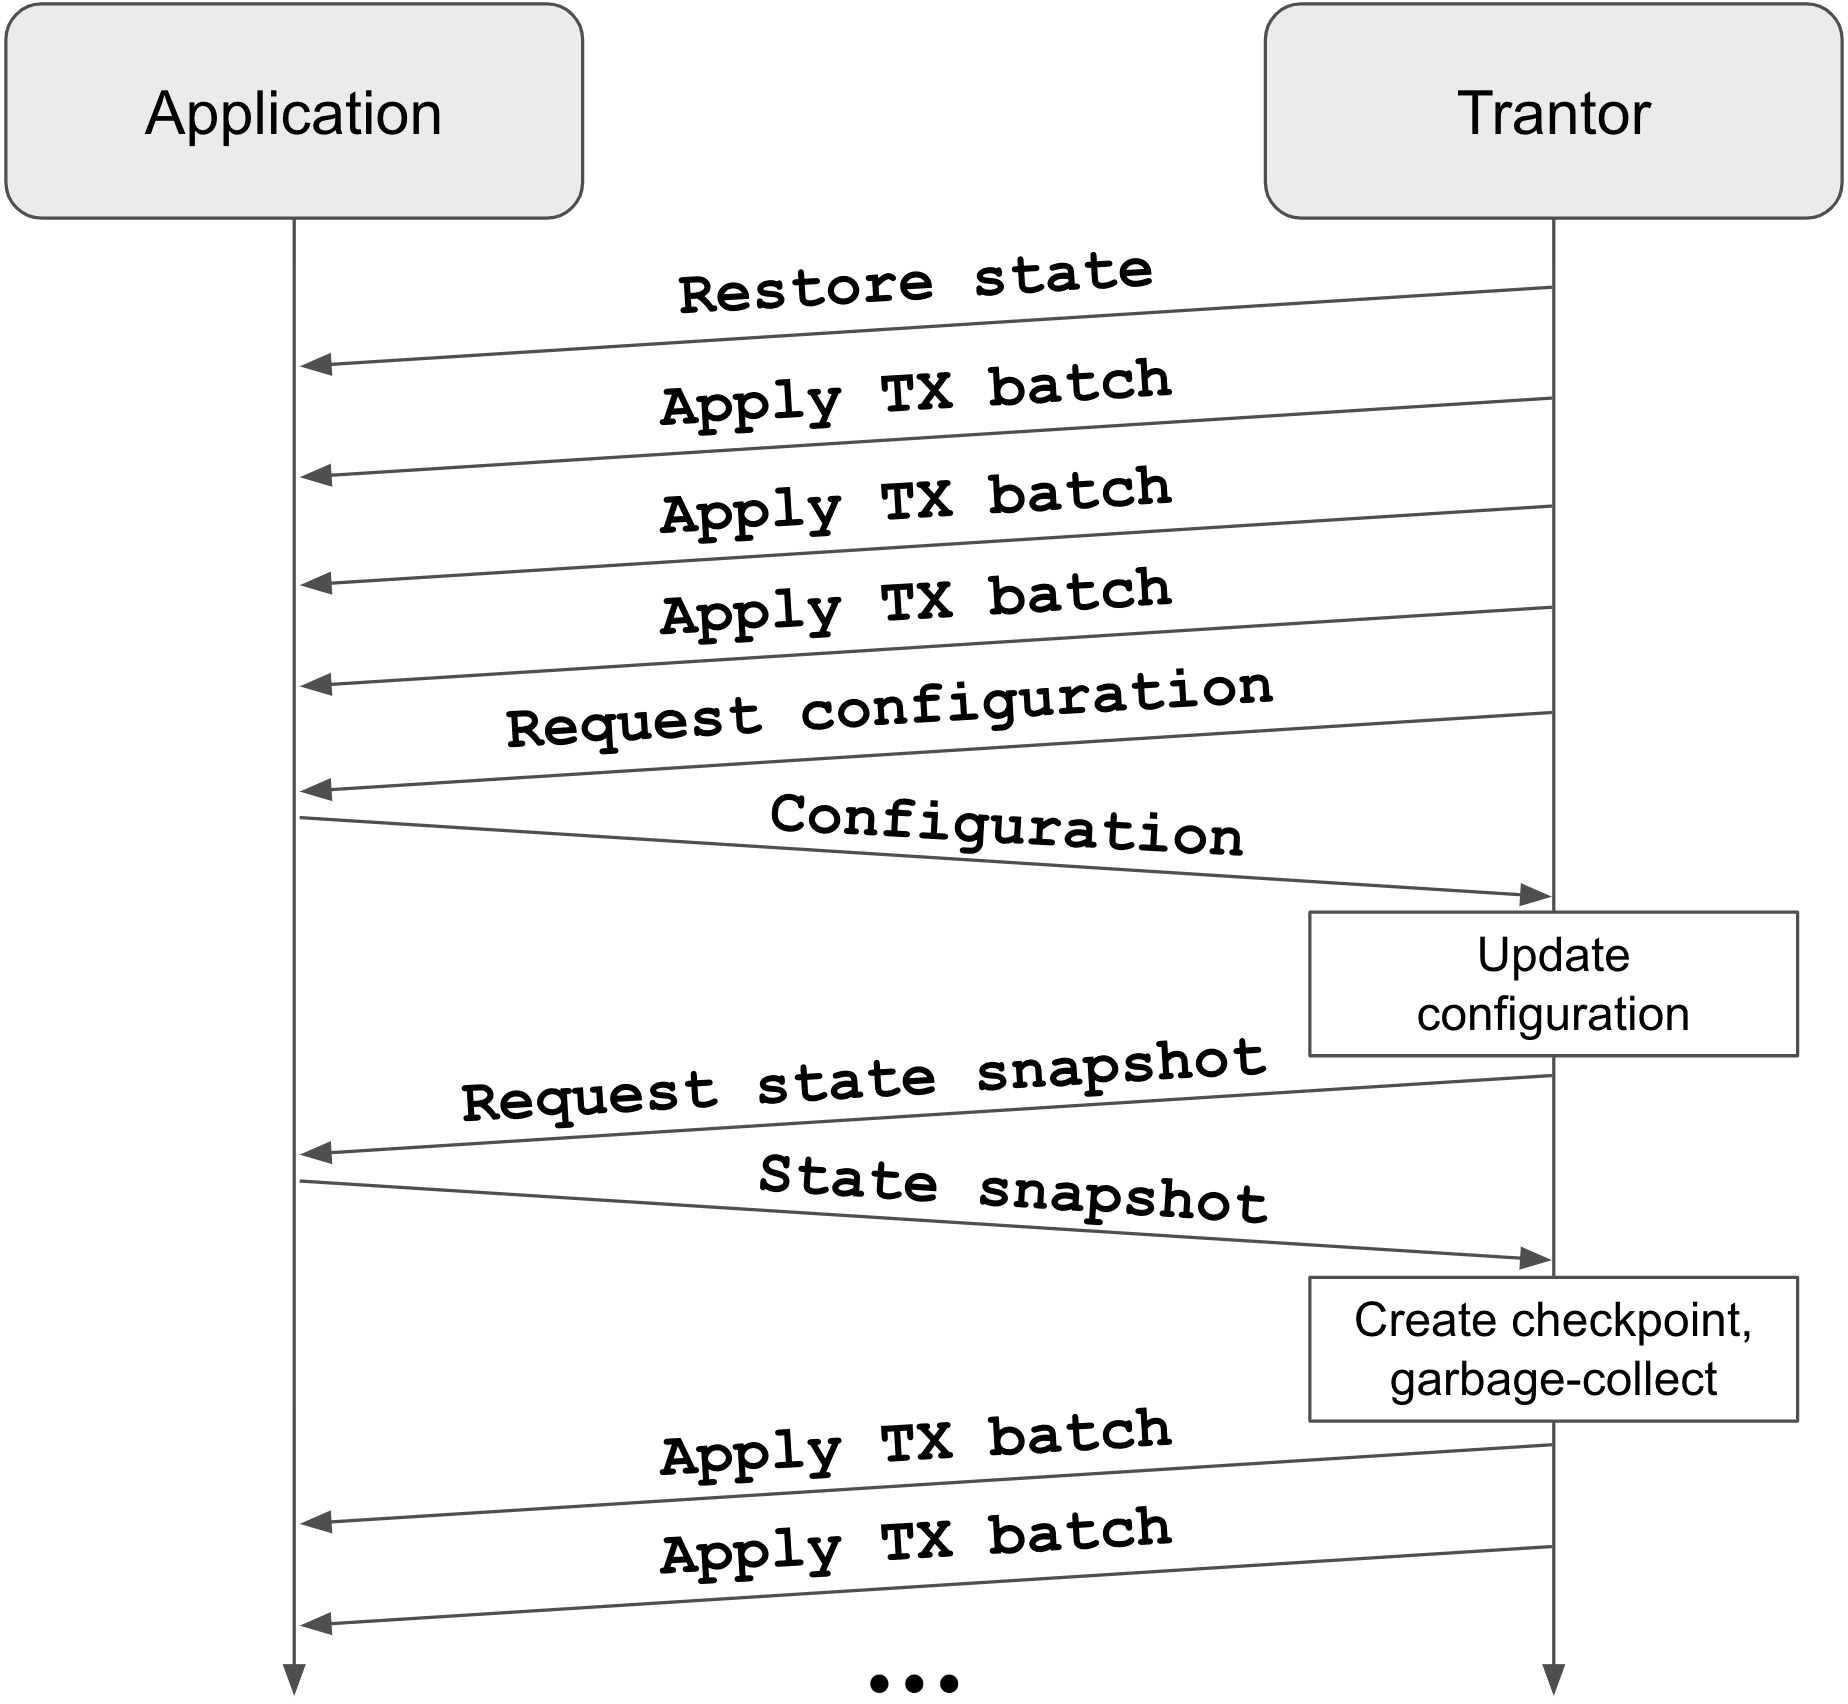
\includegraphics[width=\linewidth]{figures/application-interface.jpeg}
    \caption{Interaction between Trantor and the application it replicates.}
    \label{fig:application-interface}
\end{wrapfigure}

The set of replicas Trantor runs on can dynamically change.
Those changes are driven by the application itself, by passing the replica configuration information
(consisting of identities and network addresses of the replicas) to Trantor at run time.
The initial replica set is Trantor’s configuration parameter.
Trantor then periodically requests the next configuration from the application and parametrizes its components accordingly.

The basic interaction between Trantor and the application is similar in spirit to CometBFT’s ABCI++ interface \cite{abciplusplus}
and is depicted in \cref{fig:application-interface}.
We describe it in detail in \cref{sec:execution}.

In the rest of this document,
we briefly discuss related work in \cref{sec:related-work} and define the system model in \cref{sec:system-model}.
\Cref{sec:overview} presents an overview of Trantor’s high-level architecture and mode of operation.
In \cref{sec:algorithm-details}, we describe Trantor’s components in more detail and discuss some other noteworthy aspects of its design.
We show a preliminary performance evaluation in \cref{sec:evaluation}.
Finally, we conclude in \cref{sec:conclusions}.

\section{Related Work}
\label{sec:related-work}

Trantor proposes a decomposition of an SMR system at the conceptual level,
and follows this decomposition in its system design.
Some systems, notably Sui \cite{sui} with Bullshark \cite{bullshark} as their consensus engine,
already successfully make the point of separating transaction payload dissemination from ordering.
Hyperledger Fabric \cite{fabric} also separates execution from ordering in its execute-order-validate architecture.
Still, swapping different ordering engines is notoriously difficult and until today,
Fabric does not seem to have a proper Byzantine fault-tolerant ordering service.
Trantor takes these concepts further by treating modularity as the first priority.

CometBFT \cite{comet}, powering the Cosmos ecosystem, is an SMR system similar to Trantor in its interaction with the application.
Trantor's application interface follows a similar principle as CometBFT’s ABCI++,
more precisely, the subset of it that drives the application’s state updates.
However, ABCI++ also provides access to the application’s state, making CometBFT a proxy for querying the application state.
Moreover, CometBFT is tightly coupled with the Tendermint consensus protocol that is an integral part of the system.

\section{System Model}
\label{sec:system-model}

This section describes the basic model and assumptions Trantor uses.
In a nutshell, we consider an eventually (partially) synchronous message passing system
consisting of replicas interconnected with reliable authenticated point-to-point links.
We assume that a Byzantine adversary corrupts some of the replicas (we call those faulty)
and controls the scheduling of all network messages (within the constraints of eventual synchrony),
but cannot subvert standard cryptographic primitives, e.g., invert secure hash functions.

We generalize the usual constraint on the extent to which the adversary can corrupt replicas.
Instead of limiting their number (using the classic “f out of n” approach),
we consider each replica to be associated with a weight as part of that replica’s identity.
Roughly, the weight corresponds to the replica’s “voting power” in the system.
The total weight is the sum of the weights of all replicas.
An example of such voting power that Trantor can be parameterized with is replica stake,
as used in Proof-of-Stake protocols. 

We define a weak quorum as any set of replicas whose combined weights exceed one third of the total weight.
Analogously, a strong quorum must exceed two thirds of the total weight.%
\footnote{We could further generalize by defining the quorum thresholds arbitrarily,
as long as a weak and a strong quorum always intersect, but we stick with one third and two thirds for simplicity.}
We assume that the adversary cannot corrupt a weak quorum of replicas.
Note that, in the special case when each replica has the same weight,
our model is equivalent to the adversary corrupting less than one third of the replicas.

\section{Overview}
\label{sec:overview}

\subsection{High-Level Architecture}

We now present a simplified view of Trantor’s high-level architecture.
We intentionally leave out some details and corner cases in order to convey a high-level idea of Trantor’s general operation.
Conceptually, Trantor can be subdivided in 5 stages:

\begin{enumerate}

    \item \textbf{Mempool:} Receive transactions and group them into batches.

    \item \textbf{Dissemination:} Make transaction batches available using consistent broadcast \cite{distributedprogrammingbook} augmented by an availability certificate.
    This roughly corresponds to, making a weak quorum of replicas persistently store the batches, such that any replica can fetch them in the future.

    \item \textbf{Ordering:} Produce a totally ordered transaction log consisting of the availability certificates created at the dissemination stage.

    \item \textbf{Fetching:} Obtain the transactions using references as they appear in the transaction log.

    \item \textbf{Execution:} Apply the transactions to the application state.

\end{enumerate}

Each stage is the responsibility of a separate component that we describe below.
Logically, components communicate with other components by emitting events that other components react to.
Note that we only use the notion of events to model the interaction between Trantor's components
as is the standard in distributed system literature \cite{distributedprogrammingbook}.
We do not prescribe a particular communication model for an implementation,
even though Mir, the general framework for implementing distributed systems \cite{mir} that we use to implement Trantor,
does directly implement such an event-based model.
Alternatively (and equivalently), one can see sending an event to a component as asynchronously invoking a function of that component's interface.

\Cref{fig:basic-operation} shows a simplified diagram of Trantor’s basic operation.

\begin{figure}[h]
    \centering
    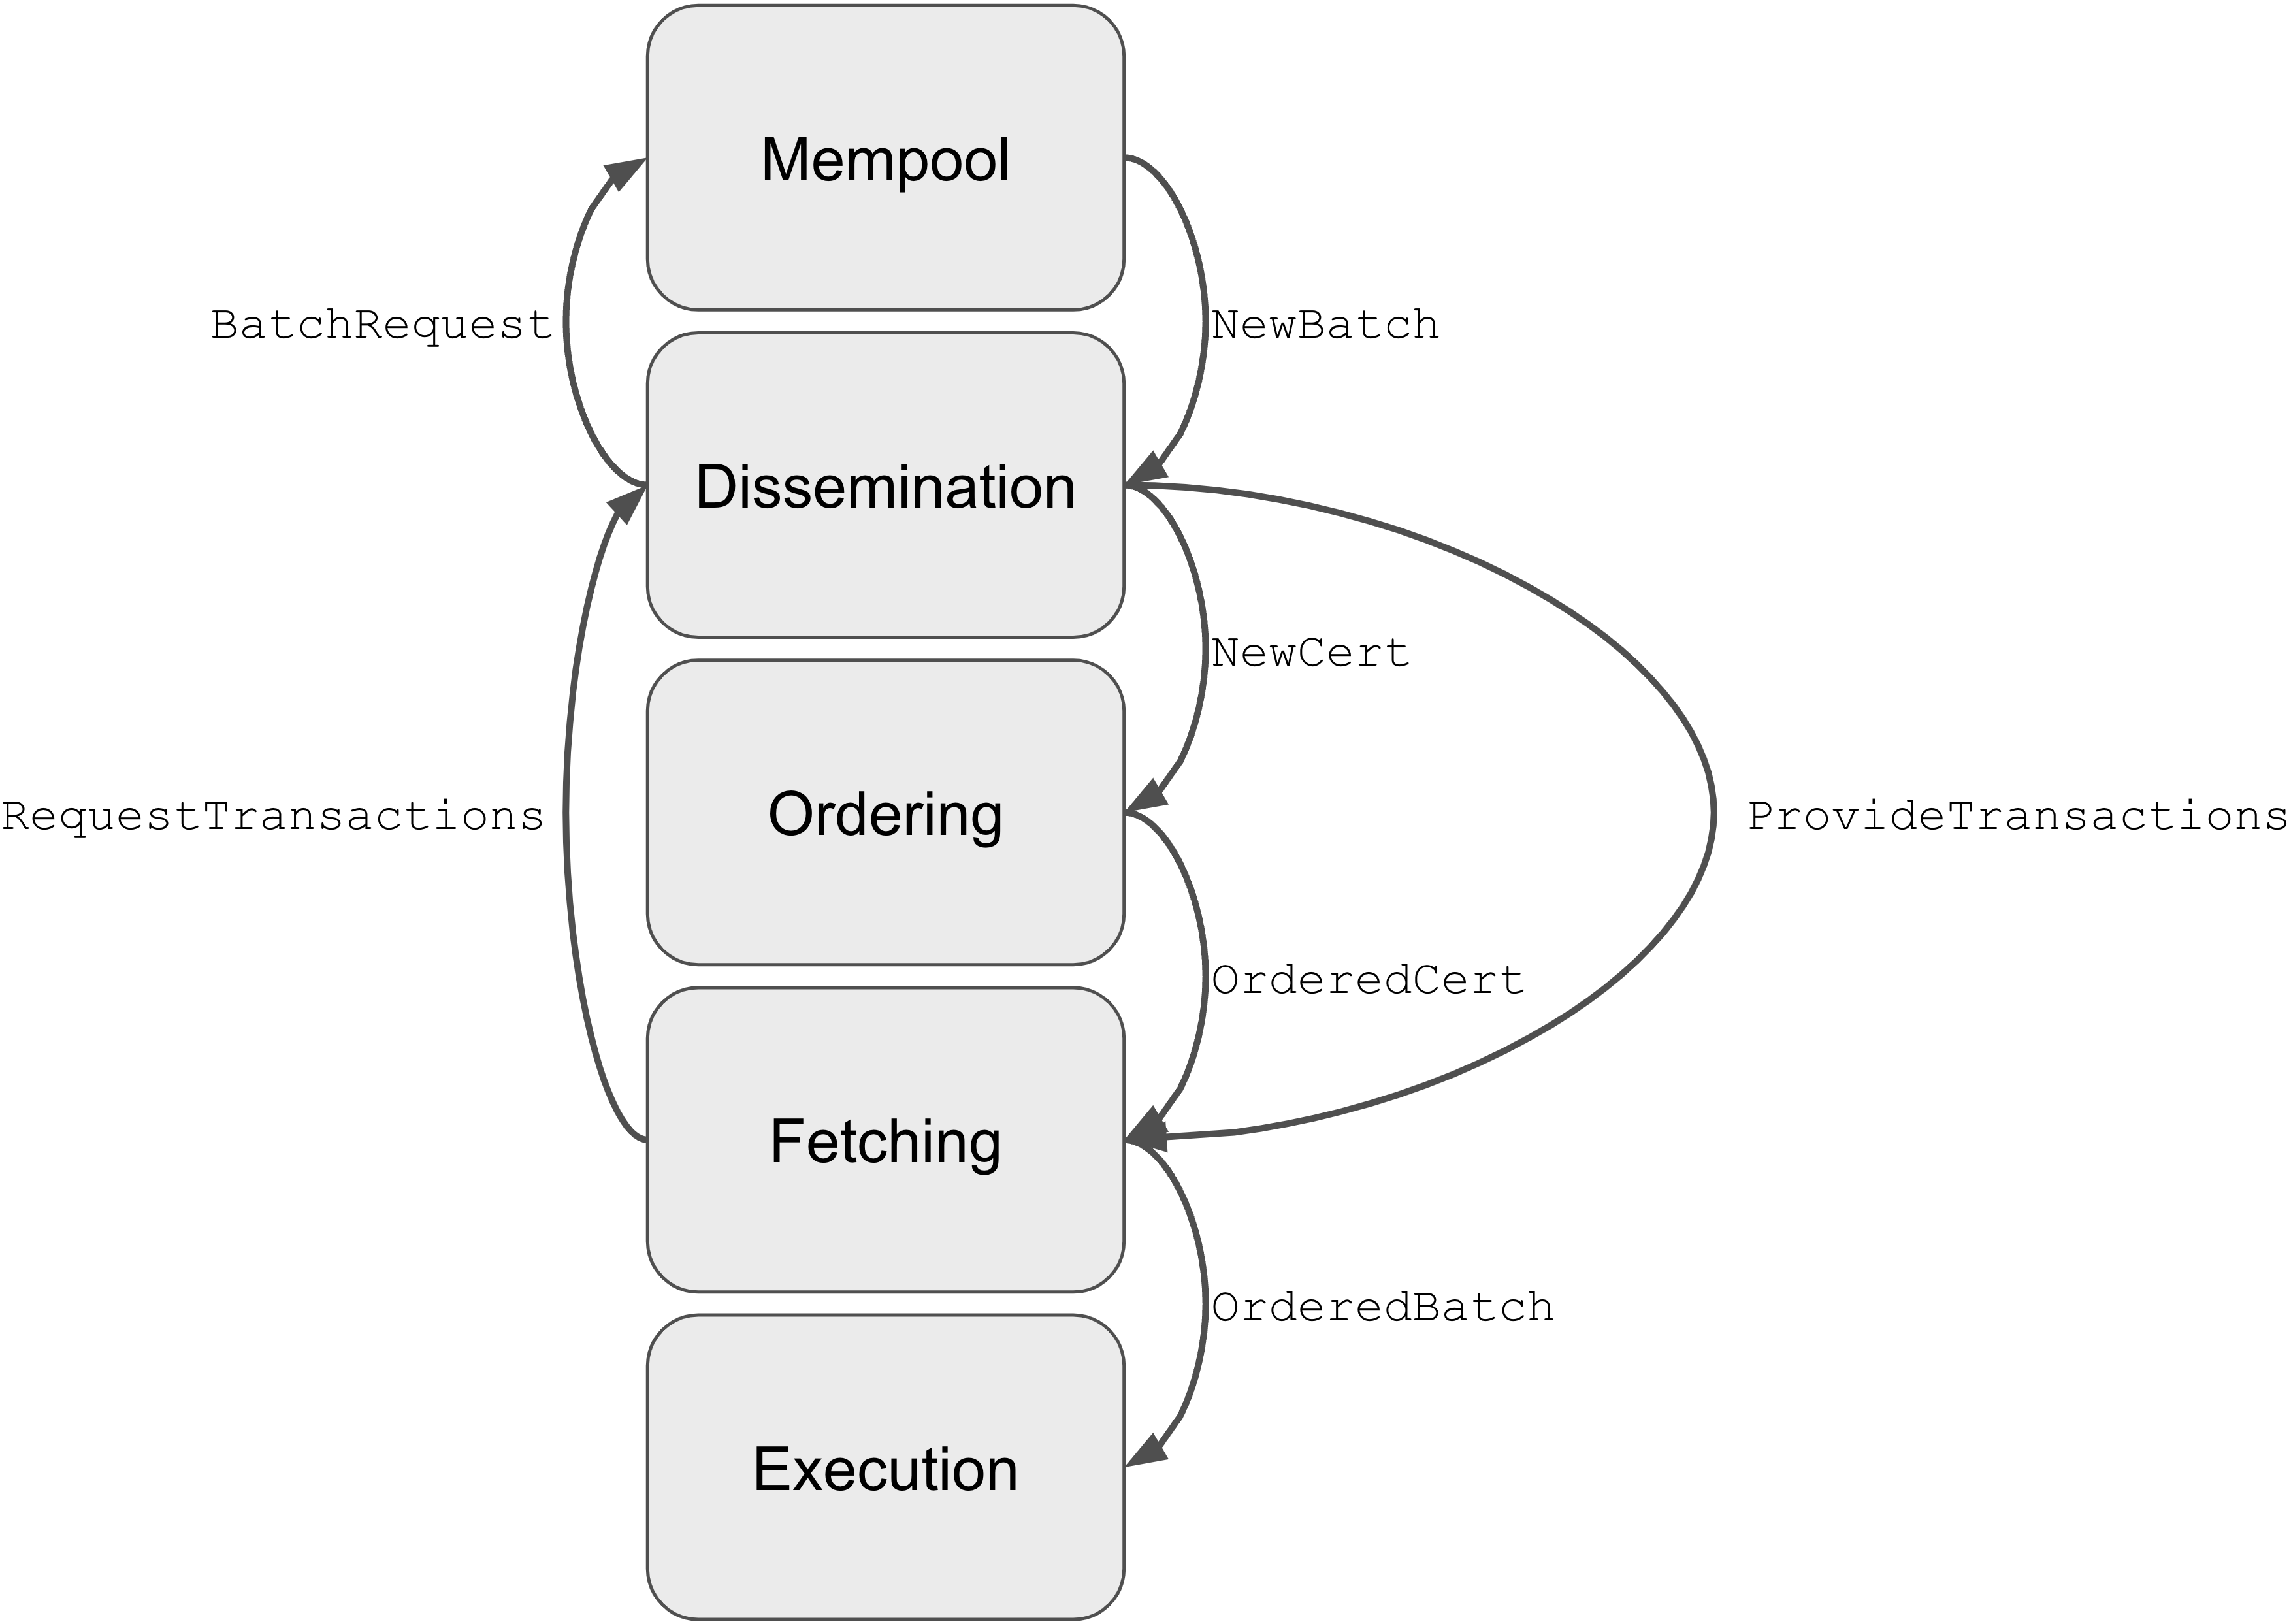
\includegraphics[width=0.8\textwidth]{figures/basic-operation.png}
    \caption{Trantor's basic operation.}
    \label{fig:basic-operation}
\end{figure}

\subsubsection{Mempool}
\label{sec:mempool}

The mempool component is responsible for transaction input.
It stores received transactions that are pending for ordering and execution.
Similarly to the application logic, we consider the mempool an external dependency
that only needs to implement an interface for interacting with the rest of the system.
Thus, how transactions are added to the mempool is out of scope of this document and,
from Trantor’s point of view, the transactions simply appear there.

It is important to note that each replica has its own local mempool
that is not expected to be consistent with other replica’s mempools.
There is no guarantee that a transaction appearing in one replica’s mempool will ever appear in another replica’s mempool.
If the same transaction does appear in multiple replicas’ mempools,
all these replicas will add their copy of the transaction to the blocks they disseminate and order.
Trantor removes such duplicates at the fetching stage (see also \cref{sec:fetching}).
Methods for removing these duplicates early on and saving resources can be implemented in a future version of Trantor.

The basic operation of the mempool is very simple.
When it receives a \event{BatchRequest} event,
it selects all the transactions that need to be proposed and responds with a \event{NewBatch} event containing those transactions.
The transactions within a batch are ordered with respect to each other.
When a batch of transactions reaches the execution stage, the transactions will be executed in this order.

\subsubsection{Dissemination}

The replica’s dissemination component has two tasks:
\begin{enumerate}
    \item Transmitting locally stored transaction batches to other replicas to ensure their global availability and
    \item Retrieving batches that are available, but not stored locally by the replica
\end{enumerate}


For ensuring transaction availability, this component obtains transactions from the mempool and broadcasts them to other replicas.
For each individual broadcast batch,
the broadcast primitive implemented by the dissemination component is that of consistent broadcast,
which ensures that no two correct replicas will observe a different batch
(i.e., prevents even faulty replicas from equivocating).
Moreover, the implementation also produces an availability certificate for each disseminated batch.
An availability certificate can be verified by any other replica and serves as a proof of global availability,
i.e., that the corresponding batch can be obtained by any correct replica using information found in the certificate.

In a nutshell, whenever the dissemination component is ready to disseminate a transaction batch,
it emits a \event{BatchRequest} event to the mempool.
Upon receiving a batch through the corresponding \event{NewBatch} event,
the dissemination component executes a protocol that sends the batch to other replicas,
asking them to persistently store it and return a signed acknowledgement.
The resulting (multisig) availability certificate then consists of a reference to (hash of) the batch
and a list of those signed acknowledgements from a weak quorum.
The dissemination component then emits the certificate in the form of a \event{NewCert} event
when requested through a \event{RequestCert} event (emitted by the ordering component).

The dissemination component’s second task is retrieving batches based on a given availability certificate.
This functionality is triggered by a \event{RequestTransactions} event containing a certificate.
Here, the component simply downloads the missing transactions from any of the replicas
that signed the certificate and emits them as a \event{ProvideTransactions} event.
Since each availability certificate is always signed by at least one correct replica, the retrieval is always guaranteed to succeed.

\subsubsection{Ordering}

The ordering component takes availability certificates produced by the dissemination component
and orders them into a sequence (called the transaction log) that is guaranteed to be the same on all replicas.
This is done using multiple parallel instances of the PBFT protocol \cite{pbft},
multiplexed together akin to the ISS protocol \cite{iss}, albeit without eliminating duplicate transactions during ordering. 

The ordering component consumes \event{NewCert} events
(containing availability certificates) produced by the dissemination component,
broadcasts (i.e., proposes) them using a total-order broadcast protocol (PBFT in our case),
and emits \event{OrderedCert} events, each representing one entry in the transaction log.

\subsubsection{Fetching}
\label{sec:fetching}

The fetching component transforms a sequence of availability certificates observed by consuming the \event{OrderedCert} events
into a corresponding sequence of transaction batches and passes them on to the execution component by producing \event{OrderedBatch} events.

In general, a significant number of the availability certificates delivered by a replica have been proposed by other replicas,
and thus the referenced transaction batches might not be present locally.
The fetching component’s task is to obtain all those batches from other replicas.
It does so by exchanging pairs of \event{RequestTransactions} / \event{ProvideTransactions} events with the dissemination component.

The fetching component also filters out transactions that have already been included in earlier batches,
such that every transaction is only passed to the execution component once (see \cref{sec:tx-deduplication}).

\subsubsection{Execution}

The execution component contains the state and logic of the application provided by the user.
It mainly consumes \event{OrderedBatch} events and applies the contained transactions to´ the application.

The execution component is also involved in checkpointing and configuring the set of replicas, which we discuss in \cref{sec:algorithm-details}.

\subsection{Epoch-Based Operation and Configuration}
\label{sec:epochs-and-configuration}

We express the progress of the whole system through the length of the transaction log.
Each ordered batch has a position in the transaction log that we call height.
Note that the whole replicated state of the system can be identified by a single number
– the height of the last applied transaction batch.
The first batch has height 0.

\subsubsection{Checkpoints}

To capture the replicated state at a certain height, Trantor uses checkpoints.
A checkpoint is a verifiable snapshot of the replicated state.
It summarizes the application of all the ordered batches up to a certain height.
We say a checkpoint is at height $h$ if it comprises the first $h$ batches of the log.
A checkpoint completely replaces a prefix of the transaction log,
i.e., a replica that obtains a checkpoint for height $h$ (summarizing batches $0$ to $h-1$)
can re-initialize its state and directly continue ordering and executing the batch at height $h$.

A checkpoint contains a certificate that any replica can verify
to confirm that the checkpointed state was indeed agreed upon.
The certificate consists of a cryptographic hash of the checkpointed state
signed by a strong quorum of replicas that agreed on that state.

\subsubsection{Epochs}

An epoch is a contiguous section of the transaction log.%
\footnote{An epoch in Trantor is not to be confused with a Filecoin epoch,
which corresponds to the notion of height in Trantor.}
Sometimes, very informally, we abuse the term epoch to also refer to the period of time
during which this section is produced (note that Trantor does not explicitly deal with the notion of time%
\footnote{Exposing a basic notion of agreed-upon real wall clock time to the application
is a feature that can be added to a future version of Trantor.}
).
An epoch has a well-defined length in terms of ordered batches.
For example, if the first epoch’s length is 4, it comprises the heights 0, 1, 2, and 3,
and the second epoch starts with height 4.
The corresponding transaction log is depicted in \cref{fig:transaction-log}.

A replica actively participates in the distributed protocols pertaining to only one epoch at a time.
Only once it fills the whole epoch’s transaction log does it advance to the next epoch.
While in principle it is possible to run multiple epochs concurrently, we stick to one epoch at a time for simplicity.

\begin{figure}[h]
    \centering
    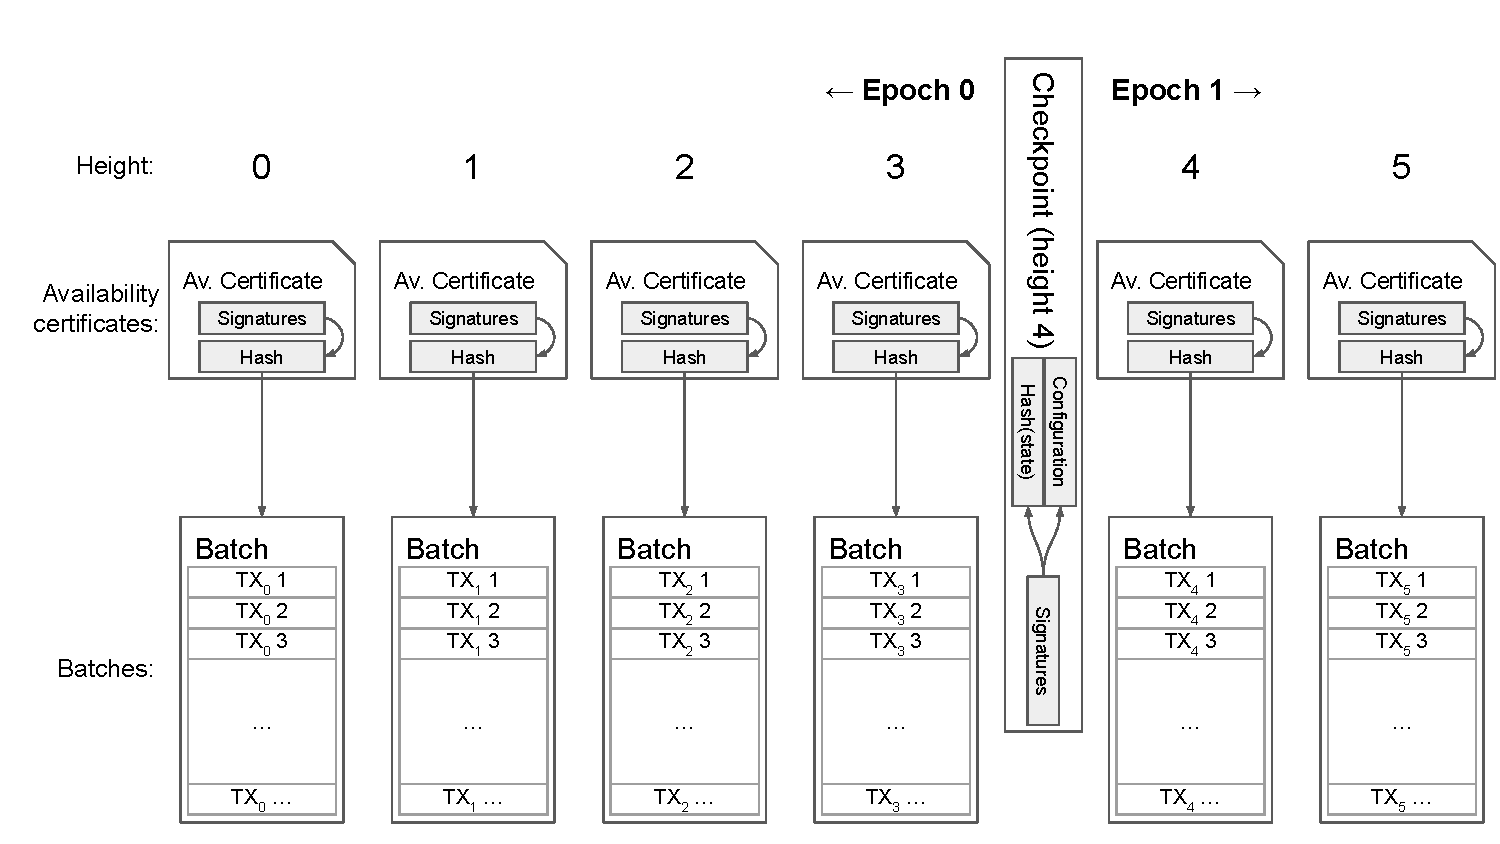
\includegraphics[width=\textwidth]{figures/transaction-log}
    \caption{The very beginning of the transaction log.
    Depicted is the first epoch of length 4, a checkpoint and the beginning of the second epoch.
    Each entry in the transaction log consists of an availability certificate (signed by a quorum of replicas)
    that refers to a transaction batch using a hash of the batch.}
    \label{fig:transaction-log}
\end{figure}

\subsubsection{Configuration}

The configuration of the whole system (including the set of replicas) is fixed throughout an epoch,
but can change from one epoch to another.
At the end of an epoch, i.e., after having applied the last transaction batch to its state,
Trantor requests a new configuration from the application (execution component) to use for future epochs.
This configuration is part of the replicated state and thus is also included in checkpoints.
Trantor creates a checkpoint at the start of each epoch,
summarizing the replicated state as it was at the end of the previous epoch.
New replicas joining the system then only need to obtain the starting checkpoint
of the first epoch the configuration of which they are part of.

To better streamline Trantor’s operation,
a configuration provided by the application at the end of epoch $e$ is not used directly in epoch $e+1$,
but rather in epoch $e+1+\param{configOffset}$, where \param{configOffset} is a system parameter.
A checkpoint thus contains the configuration for not just the epoch it starts,
but also for \param{configOffset} additional subsequent epochs.
Correspondingly, Trantor uses the initial configuration for the first $\param{configOffset}+1$ epochs.

\section{Algorithm Details}
\label{sec:algorithm-details}

This section describes the algorithms we use to implement Trantor’s components in more detail
and explains some additional noteworthy aspects of Trantor’s design.

\subsection{Dissemination}

In each epoch, a subset of Trantor’s replicas are designated as leaders by the ordering component
(see MirBFT \cite{mirbft} and ISS \cite{iss} for details).
Each leader replica’s dissemination component continuously executes the following simple algorithm.

\begin{enumerate}
\item Emit a \event{BatchRequest} event to the mempool.
\item Wait for obtaining a transaction batch through the corresponding \event{NewBatch} event from the mempool.
\item Send a \msg{RequestSig} message to all other replicas (including itself), containing the obtained batch.
\item Upon reception of a \msg{RequestSig} message,
persistently store the transaction batch and sign a digest of all its contents
(our implementation uses ECDSA over the Secp256k1 curve).
\item Respond with a \msg{Sig} message containing the computed signature.
\item Upon reception of valid signatures from a weak quorum (including itself),
construct a multisig availability certificate out of those signatures and the batch digest,
and store the certificate in a buffer.
(A weak quorum of signatures ensures that there is at least one correct replica the data can be fetched from later,
making the batch available.)
\item If the buffer is not yet full, restart from 1.
\end{enumerate}

Upon reception of a \event{RequestCert} event from the ordering component,
the dissemination component responds with a \event{NewCert} event
containing all the availability certificates present in its buffer, empties the buffer,
and restarts the above dissemination algorithm in case it has stopped due to a full buffer.

With this approach, many multisig certificates are contained in a single \event{NewCert} event.
This allows for a continuous dissemination of transaction batches
even before the ordering component requests any certificates.
Once a \event{RequestCert} event arrives, the ordering component can respond immediately with the buffered certificates
and the ordering can start without further delay.

The size of the buffer is a configuration parameter
and also determines the maximal number of multisig certificates contained in one NewCert event.
For simplicity, we refer to such a batch of certificates as a single availability certificate
downstream from the dissemination component.
Any operation applied to it is, under the hood, applied to all the sub-certificates.
We consider an availability certificate valid iff all the contained sub-certificates are valid.

\subsection{Ordering}

Trantor’s ordering component establishes a total order on availability certificates
received from the dissemination component using a protocol that multiplexes multiple instances of PBFT.
It is inspired by the ISS protocol \cite{iss}, but forgoes transaction deduplication for simplicity
(it can be added in a future version of Trantor).

In short, at the start of each epoch, Trantor assigns each height of that epoch to one leader replica
and initializes one instance of PBFT per leader.
The leader is configured to be the first PBFT primary charged with proposing availability certificates
for all the heights (“sequence numbers” in PBFT terminology) assigned to it.

The liveness of each individual PBFT instance guarantees
that each height will eventually be assigned an availability certificate.
If the leader fails (or there is asynchrony in the network),
the remaining correct replicas agree on a special empty certificate (that does not refer to any transactions) instead. Once all heights of an epoch have been assigned availability certificates,
Trantor advances to the next epoch, repeating the whole process.
For details on the ordering protocol, we refer the interested reader to ISS \cite{iss}.

\subsection{Creating Checkpoints}

The creation of checkpoints is performed by a dedicated sub-protocol, but is orchestrated by the ordering component.
Immediately after a transition from epoch $e-1$ to $e$, before any batches are appended to the transaction log,
the ordering component creates a new instance of the checkpointing protocol,
parametrized with a snapshot of the system state comprised of:
\begin{compactitem}
\item The current state of the application as obtained from the execution component
\item Relevant state of the Trantor protocol itself,
such as epoch number, height, and other variables that need to be reinitialized when restoring the state
\item Configuration of epoch $e$ and the \param{configOffset} following epochs
\item Information about processed transactions (needed for deduplication, see \cref{sec:tx-deduplication})
\end{compactitem}
Each replica of epoch $e-1$ then executes a simple checkpointing protocol akin to the one used in PBFT:
\begin{enumerate}

\item Compute a digest of the snapshot and sign it.

\item Send the signed digest to all other replicas.

\item Wait for the reception of matching signed digests from a strong quorum%
\footnote{Using a weak quorum would be sufficient under our assumptions,
since it would still guarantee a correct replica storing a provably correct (thanks to the certificate) checkpoint.
However, since we use checkpoints as a condition for a replica to advance epochs,
requiring a strong quorum limits the number of slow replicas that can fall behind to less than a weak quorum.}
(including self).

\item Construct a (multisig) checkpoint certificate from the snapshot digest and the collected signatures.

\item The checkpoint itself consists of the state snapshot and the checkpoint certificate.

\end{enumerate}

Once the checkpoint is ready, the ordering component saves it in its state, replacing any older checkpoints.
Moreover, the ordering component also informs the application (execution component) about the new checkpoint.
This can be useful to the application for various reasons, e.g., creating backups consistently with other replicas.

Note, however, that the constructed checkpoint certificates, all being valid,
may contain different signatures on different replicas.
In other words, each replica may create a different valid certificate,
depending on which signatures the replica received first.
In order to adhere to the paradigm of providing identical inputs to all copies of the application on all replicas,
Trantor creates another instance of a consensus protocol (also PBFT in our case)%
\footnote{In our modular implementation of Trantor, we use (different instances of) the very same PBFT module
to agree on both availability certificates and checkpoints - an example of the benefits of modularity.}
to agree on one single version of the certificate.
This certificate is then used by all replicas for the checkpoint delivered to the application.

\subsection{Garbage Collection and State Transfer}
\label{sec:garbate-collection-state-transfer}

A checkpoint for epoch $e$ (i.e, appearing between epochs $e-1$ and $e$ in the transaction log)
contains all information necessary for a replica to start / continue operating from the beginning of epoch $e$.
Thus, as soon as such a checkpoint is available to a replica, it garbage-collects all data related to earlier epochs.
The rationale is that the effect of any message that would need to be sent for any of the previous epochs is subsumed by the checkpoint which,
if needed, can be transmitted instead.

Any replica that falls behind (e.g., due to transient network failures or simply due to being slow) can completely recover its state from a checkpoint.
To this end, each replica keeps track of the highest epoch it observed in communication received from each other replica.
When a replica $r$ notices the epoch of another replica $r'$ being lower by a predefined threshold (Trantor’s system parameter),
$r$ sends its latest checkpoint to $r'$.
$r'$ does not need to wait for any quorum to confirm the validity of the checkpoint, as it can verify the received checkpoint’s certificate.

Note that this naive state transfer algorithm is correct, but rather inefficient,
as it leads to multiple correct replicas sending the same checkpoint (a potentially bulky data structure) to the same straggling replica.
This inefficiency can easily be optimized away by only notifying the straggler about the own progress
and letting the straggler request the checkpoint data from only one replica at a time (or even request chunks of it from multiple replicas).
Another possibility is storing the checkpoint in an external data store available to all replicas
and only transfer a reference (e.g., an IPLD pointer) to it between replicas.

Since checkpoint (multisig) certificates consist of a list of signatures, the verification relies on the knowledge of the signers’ public keys.
If the set of replicas (i.e., membership) never changes, all replicas can easily verify checkpoint certificates
based on their knowledge of all other replica’s public keys.
If, however, we want to allow the system to dynamically reconfigure the membership (see \cref{sec:execution})
and, at the same time, not place any assumptions on the correctness of replicas removed from the replica set,
verifying checkpoint certificates becomes more difficult due to possible long-range / ``i still work here'' attacks \cite{longrangeattacks}.
Handling this case exceeds the scope of this document and will be added to a future version of Trantor.%
\footnote{If Trantor is used in an IPC \cite{ipc} subnet, for example, the parent subnet within the IPC hierarchy can naturally serve as a trusted source of membership information.}

\subsection{Transaction Identification and Post-Order Deduplication}
\label{sec:tx-deduplication}

In order to apply each transaction exactly once, Trantor needs to keep track of which transactions have been applied in the past.
To this end, each transaction is uniquely identified by a tuple (\textit{ClientID}, \textit{TxNo})
with ClientID uniquely identifying the entity that created the transaction (the client), e.g., a user of the system.
The transaction number \textit{TxNo} is a number that each client assigns to each transaction it produces.
The client is responsible for producing transactions with monotonically increasing \textit{TxNo}s.
If two transactions with different payloads but the same \textit{TxNo}s are produced by the same client,
Trantor does not guarantee processing any of them.
One (not both) of them, however, still might be applied.

Trantor uses these transaction identifiers at the fetching stage to filter out transactions that have already been executed previously.
For each client, Trantor keeps an entry for all \textit{TxNo}s passed to the execution component.
When the fetching component obtains a batch of transactions from the dissemination component, it filters out those for which an entry already exists.

The data structures required by such a simple filter, however, would grow indefinitely and eventually exhaust all the system’s resources.
We therefore introduce the concept of a client watermark window - a range of \textit{TxNo}s a client is allowed to concurrently submit to the system.
If a transaction outside of the client’s watermark window appears in the mempool, Trantor is allowed to ignore it.
At each epoch transition, Trantor sets the start of each known client’s watermark window to the lowest \textit{TxNo} not yet executed.
The window then extends over the next \param{WindowSize} transaction numbers, where \param{WindowSize} is a system parameter.

Leveraging the client watermark window, Trantor only needs a constant amount of memory to represent
all transactions ever executed that originate from a single client.
The total memory overhead is thus $O(c)$, $c$ being the number of clients.
Reducing this overhead even further is possible under some mild additional synchrony assumptions by garbage-collecting information about inactive clients,
but is out of the scope of this document and may be implemented in a future version of Trantor.

\subsection{Execution}
\label{sec:execution}

The execution component is responsible for managing the application state and execution. Its tasks are the following.

\begin{itemize}
    \item Apply transactions contained in ordered batches to the application logic.
    \item Consume periodically generated checkpoints.
    \item Create snapshots of the application state.
    \item Restore the application state from snapshots.
    \item Dynamically configure the Trantor system (e.g., define the replica membership).
\end{itemize}

The application logic is an external dependency that Trantor’s execution component simply relays events to.
For convenience, Trantor supports two variants of the application logic: a simplified static one and a full-fledged one with reconfiguration support.

\subsubsection{Simple Static Application}

The simple static variant only needs to implement the following functions:

\begin{itemize}
    \item \code{ApplyTXs(transactions)}: Applies a batch of transactions to the state machine.
    \item \code{Snapshot() \textrightarrow{} serialized\_state}: Returns a snapshot of the application state.
    \item \code{RestoreState(checkpoint)}: Restores the application state from a checkpoint.
    \item \code{Checkpoint(checkpoint)}: Announces a new checkpoint to the application.
\end{itemize}

The Snapshot and RestoreState functions are tightly coupled; what Snapshot returns, RestoreState must be able to parse.
The \code{serialized\_state} value (represented as an opaque byte array) returned by Snapshot
will be contained (as one of the fields) in the checkpoint that Trantor passes to RestoreState
(other fields contain additional metadata such as the checkpoint certificate).
The application thus has full control over serializing and deserializing its own state.
This means, in particular, that a large application state need not necessarily be all encoded in the value returned by Snapshot,
but can be, for example, a reference to an external data store (e.g., IPFS) that stores the actual state and to which all replicas have access.

The Checkpoint function is technically not necessary for implementing a textbook version of state machine replication
and can safely be ignored by an application implementation that does not make use of checkpoints.
In practice, however, this feature can be useful, e.g., for backup purposes.

\subsubsection{Reconfigurable Application}

Applications that wish to be able to dynamically reconfigure the Trantor system can use the full-fledged application interface.
On top of the simple one, the full-fledged application interface contains one additional function:
\begin{itemize}
    \item \code{NewEpoch(number) \textrightarrow{} configuration}: Announces the start of a new trantor epoch with number number.
    Returns a configuration to be used by Trantor after \param{configOffset} epochs.
\end{itemize}

We expect the decisions on new configurations to be made by the replicated application logic, based only on the replicated state.
Since Trantor consistently invokes the \code{NewEpoc}h function after having applied the same sequence of transactions on each replica,
we ensure that the configuration decisions will be consistent across different copies of the application at all correct replicas as well.

\subsubsection{Example Execution}

To illustrate the operation of the execution component,
\cref{lst:example-execution} shows the sequence of application function invocations as they would appear at each replica in a system with epoch length 4,
corresponding to the transaction log depicted in \cref{fig:transaction-log}.
\begin{lstlisting}[
  mathescape,
  basicstyle=\ttfamily,
  columns=fullflexible,
  frame=lines,
  xleftmargin=0.2\textwidth,
  xrightmargin=0.2\textwidth,
  aboveskip=1em,
  belowskip=1em,
  framexleftmargin=0.1\textwidth,
  framexrightmargin=0.1\textwidth,
  framexbottommargin=1em,
  framextopmargin=1em,
  label=lst:example-execution,
  captionpos=b,
  caption= Application of the application corresponding to \cref{fig:transaction-log}.
]
 1. NewEpoch(0)
 2. ApplyTXs(TX$_0$1, TX$_0$2, ...)
 3. ApplyTXs(TX$_1$1, TX$_1$2, ...)
 4. ApplyTXs(TX$_2$1, TX$_2$2, ...)
 5. ApplyTXs(TX$_3$1, TX$_3$2, ...)
 6. Snapshot()
 7. Checkpoint(checkpoint)
 8. NewEpoch(1)
 9. ApplyTXs(TX$_4$1, TX$_4$2, ...)
10. ApplyTXs(TX$_5$1, TX$_5$2, ...)
11. ...
12. ...
\end{lstlisting}

The purpose of Trantor can be summarized as ensuring that exactly his sequence of application invocations happens consistently at all replicas,
regardless of transactions appearing in the mempools in different orders and some replicas failing or even misbehaving.

Note that Trantor does not invoke the \code{RestoreState} function under normal circumstances.
It is only invoked on replicas that fall behind and need to catch up, or on replicas that freshly joined the system after reconfiguration.
The application must be ready to receive such an invocation at any point in time.
Trantor guarantees, however, that the restoration happens at epoch boundary,
i.e., Trantor only restores a snapshot taken at the end of an epoch, before any transactions from the next epoch have been applied.
The standard sequence of invocations from the start of an epoch then follows (unless state needs to be restored again), as in \cref{lst:restoring-state}.

\begin{lstlisting}[
  mathescape,
  basicstyle=\ttfamily,
  columns=fullflexible,
  frame=lines,
  xleftmargin=0.2\textwidth,
  xrightmargin=0.2\textwidth,
  aboveskip=1em,
  belowskip=1em,
  framexleftmargin=0.1\textwidth,
  framexrightmargin=0.1\textwidth,
  framexbottommargin=1em,
  framextopmargin=1em,
  label=lst:restoring-state,
  captionpos=b,
  caption=Restoring application state from checkpoints.
]
 1. NewEpoch(0)
 2. ApplyTXs(TX$_0$1, TX$_0$2, ...)
 3. ApplyTXs(TX$_1$1, TX$_1$2, ...)
 4. ApplyTXs(TX$_2$1, TX$_2$2, ...)
 5. RestoreState(checkpoint)
 6. RestoreState(checkpoint)
 7. NewEpoch(8)
 8. RestoreState(checkpoint)
 9. NewEpoch(532)
10. ApplyTXs(TX$_{...}$1, TX$_{...}$2, ...)
11. ApplyTXs(TX$_{...}$1, TX$_{...}$2, ...)
12. ...
13. ...
\end{lstlisting}

\section{Implementation}
\label{sec:implementation}

We now present our implementation of Trantor, diving deeper into Trantor's architecture and refining the descriptions from \cref{sec:overview,sec:algorithm-details}.
We implement Trantor in Go, using the Mir distributed system implementation framework \cite{mir}.
Note that we are describing the implementation of a \emph{single replica}.
Each replica runs its own copy of what we present in this section.
In the following, we first explain some overarching concepts relevant for all modules and then describe each module in detail.

\subsection{Epochs}

As mentioned in \cref{sec:epochs-and-configuration}, Trantor's operation is epoch-based.
Therefore, several components are, explicitly or implicitly, associated with a concrete epoch.
The \module{Orchestrator} module drives progress from one epoch into the next one.
It instantiates and initializes all the modules necessary for an epoch, assembles the corresponding part of the event log from their output,
triggers the creation of a checkpoint, and, when the checkpoint is available, triggers garbage collection.

Several modules in \cref{fig:implementation-diagram} (\module{Dissemination}, \module{Ordering}, \module{Checkpointing}) contain submodules.
While the top-level modules are long-lived and exist throughout Trantor's operation,
the submodules are generally only relevant for one epoch, for which the \module{Orchestrator} dynamically instantiates them, and are eventually garbage-collected.

\subsection{Garbage Collection Using the Retention Index}

In Trantor, garbage collection is very explicit.
Each data structure (including whole submodules) that is subject to garbage collection is explicitly associated with an integer \emph{retention index}.
The retention index is a system-wide, monotonically increasing variable driven by the \module{Orchestrator}.
All data associated with a retention index lower than the current one is defined to be obsolete and safe to delete.
In Trantor, the retention index is derived from the epoch number,
resulting in the garbage collection semantics described in \cref{sec:garbate-collection-state-transfer}.

We could have performed garbage collection directly based on the epoch number,
but using the retention index helps keep the semantically different concepts ``progress in SMR'' and ``garbage collection'' cleanly separated.
This way, modules that otherwise do not have a reason to be aware of the progress of the whole state machine (or even of the concept of SMR)
-- which are, in fact, most of the modules --
can be cleaner, simpler, more general, and thus more reusable.

\begin{figure}[h]
    \centering
    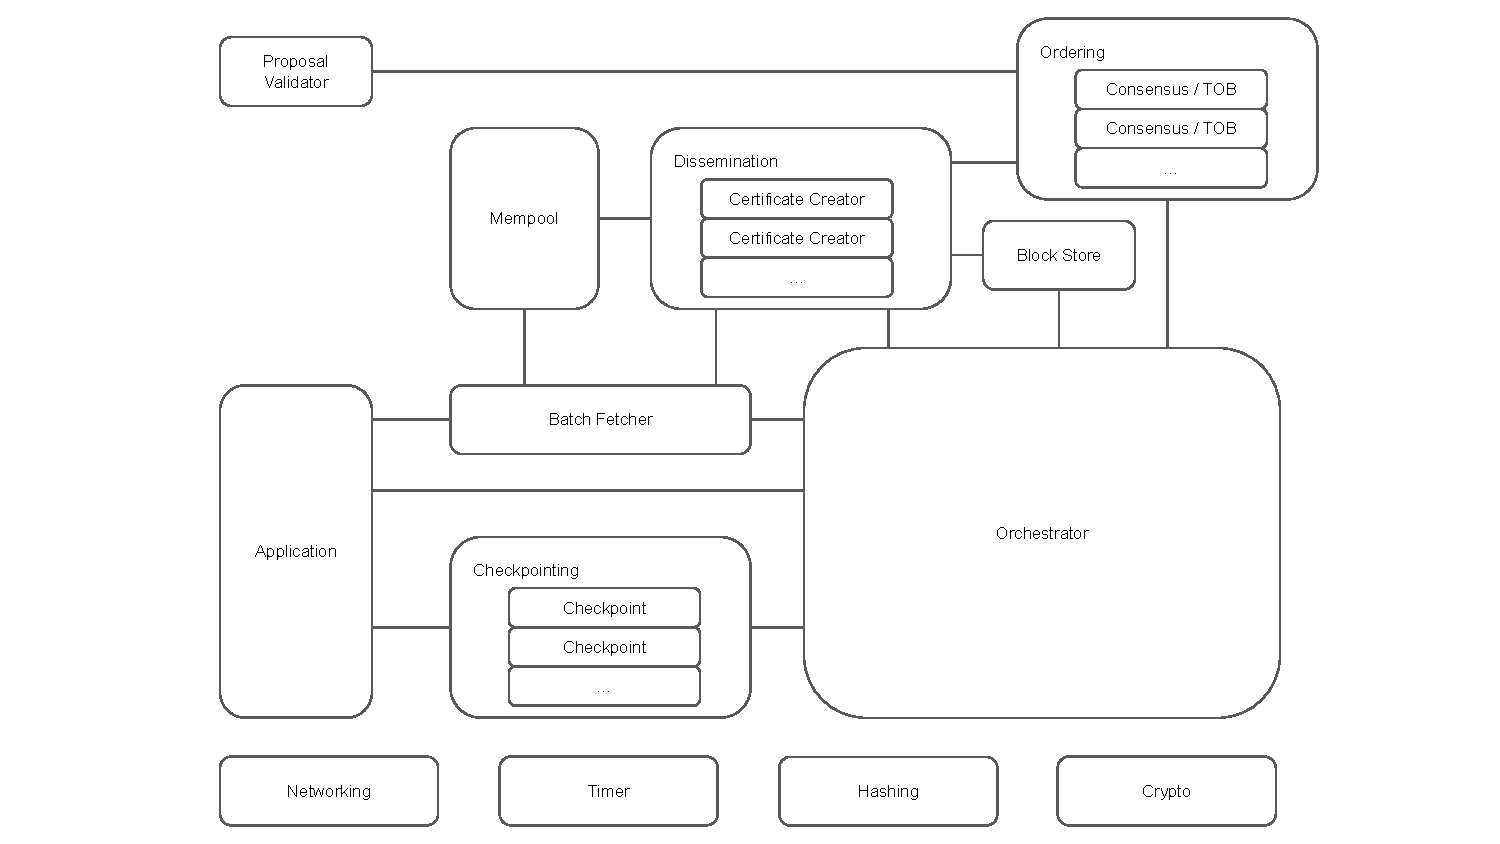
\includegraphics[width=\textwidth]{figures/implementation-diagram}
    \caption{Schematic view of Trantor's implementation's components.
    A line between two boxes means that the two components interact.
    The four bottom-most components (\module{Networkig}, \module{Timer}, \module{Hashing}, and \module{Crypto}) have a supporting role.
    They interact with many other components and we omit the corresponding lines in the diagram for simplicity of presentation.}
    \label{fig:implementation-diagram}
\end{figure}

\subsection{Trantor's Modules}

\Cref{fig:implementation-diagram} displays all relevant modules of Trantor's implementation and their interactions.
It rather accurately represents the structure of our code, omitting only few technical details not relevant for understanding the workings of the implementation.
To improve the presentation, the names of some events and modules also do not necessarily fully correspond to those used in the code.

\subsubsection{\module{Orchestrator}}

The \module{Orchestrator} is the heart (and brain) of Trantor.
Its main task is to advance the transaction log.
In addition to the transaction log data structure, the \module{Orchestrator} maintains the configurations
(including replica membership information) of the current and \param{ConfigOffset} next epochs,
as well as the most recent checkpoint.
It also keeps track of the progress of other replicas in order to decide when they need to be sent a checkpoint to catch up.

Trantor always starts operating from an initial checkpoint (equivalent to a genesis block in some other blockchain systems),
with which the \module{Orchestrator} is initialized.
A checkpoint, by definition, defines the system state at the start of an epoch.
Upon initialization, the \module{Orchestrator} thus initializes all its internal data structures
and emits events other modules corresponding to the start of a new epoch.
This includes instructing the \module{Dissemination} and \module{Ordering} modules to create new submodules
executing, respectively, the dissemination and ordering protocols for the new epoch.
The \module{Orchestrator} then waits for events from the \module{Ordering} module announcing the delivery of availability certificates
for all the heights of the epoch, which it relays (in the correct order) to the \module{Block Fetcher}.

At any point in time, the \module{Orchestrator} may receive a \event{RestoreFromCheckpoint} event,
in which case it performs a re-initialization as described above, using the received checkpoint.

The \module{Orchestrator} consumes the following events:
\begin{itemize}
    \item 
\end{itemize}

\section{Performance Evaluation}
\label{sec:evaluation}

This section presents a preliminary performance evaluation of Trantor, measuring the latency and throughput of ordering transactions.
The purpose is not to improve upon the state of the art in any particular metric,
but rather show that Trantor can provide more than sufficient throughput (tens of thousands oft transactions per second)
and acceptable latency (sub-second in a global deployment) for many real-world applications.
Most importantly, we show that the performance price for modularity and clean abstractions is worth paying.

For now, we only evaluate the "good-case" performance, that is, we do not artificially introduce faults or simulate Byzantine behavior of some replicas.
Mechanisms for dealing with such situations are in place, however (PBFT view change),
and we plan on evaluating Trantor's performance under adverse conditions in the future.

\subsection{Experimental Setup}

We measure Trantor's performance at a moderate scale of 32 and 64 replicas.
For each replica, we use an Amazon EC2 virtual machine of type \texttt{t4g.xlarge}
with 4 virtual Arm-based AWS Graviton2 CPUs and 16GB of memory (even though most of the memory is not used).
The replicas are either all connected by a local network (LAN) or dispersed over the globe as far apart as possible, communicating over the internet (WAN):
\begin{compactitem}
    \item \textbf{LAN:} Single Amazon datacenter in Ireland.
    \item \textbf{WAN:} 8 Amazon datacenters:
    N. Virginia (\texttt{us-east-1}),
    N. California (\texttt{us-west-1}),
    Seoul (\texttt{ap-northeast-2}),
    Sydney (\texttt{ap-southeast-2}),
    Central Canada (\texttt{ca-central-1}),
    Frankfurt (\texttt{eu-central-1}),
    Ireland (\texttt{eu-west-1}),
    and Sao Paulo (\texttt{sa-east-1}).
\end{compactitem}
For the WAN deployments, replicas are uniformly distributed among the 8 different locations,
i.e., 4 replicas and 8 replicas in each location respectively for deployments of 32 and 64 replicas.

\subsection{Mempool Implementation}

While, as mentioned in \cref{sec:mempool}, the design of Trantor treats the mempool as an external dependency,
our implementation includes a mempool module that accepts \event{NewTransaction} events and stores the contained transactions in memory.
Upon receiving a \event{RequestBatch} event, the mempool responds with a \event{NewBatch} event containing the stored transactions.
The mempool's operation is influenced by several parameters:

\begin{itemize}
    
    \item \param{MaxTransactionsInBatch}: An emitted \event{NewBatch} event never contains more than \param{MaxTransactionsInBatch} transactions.
    If the number of stored transactions exceeds this value, the next emitted batch will contain the \param{MaxTransactionsInBatch} least recently added transactions.
    In our experiments, we always use a value 2048 for this parameter (chosen empirically after exploring a few others).
    
    \item \param{MaxPayloadInBatch}: Analogously to \param{MaxTransactionsInBatch},
    \param{MaxPayloadInBatch} defines the maximal total cumulative payload size of all transactions in a batch.
    We use a very large value of 16MB in our experiments to effectively disable this limit.
    
    \item \param{BatchTimeout}: To enable effective batching of transactions, the mempool does not respond to a \event{BatchRequest} immediately
    if there are not enough pending transactions for reaching at least one of the two above limits.
    \param{BatchTimeout} defines the maximal time the mempool waits for a batch to fill.
    After \param{BatchTimeout} elapses, the mempool emits a \event{NewBatch}, even if it is not full (or is even completely empty).
\end{itemize}

\subsection{Load Generation Generation and Data Collection}

To generate the load, we implement simple clients that generate transactions and insert them into the replicas' mempools.
To measure purely the throughput and latency of transaction ordering, we co-locate each client with a replica on the same machine.
In fact, each client is merely a thread within the replica's process.%
\footnote{Trantor's design is very well-suited to implement such clients --
one merely needs to add a module continuously producing \event{NewTransaction} events consumed by the mempool.}

The clients operate in a “closed loop”.
Each client submits a transaction with 512 bytes of randomly generated payload, waits until the transaction is delivered, and then immediately submits the next one.
We consider a client's transaction \textit{tx} delivered when the replica the client is located on invokes \code{ApplyTX(transactions)} with $tx \in \code{transactions}$.
In our experiments, we gradually increase the number of such clients until the system becomes saturated and the throughput stops increasing.
Most of the time, it takes tens of thousands of clients to saturate the system.

The duration of each run (corresponding to one data point in the plots) is 2 minutes.

\subsection{Latency Metrics}

This preliminary evaluation focuses on the expected "good-case" scenario that users might expect during normal operation of the system.
We conduct our experiments in a simple way, gathering the data during the whole 2 minutes of each experiment's duration.
As is common in experiments where not all replicas can start up at exactly the same time,
the data from the first and last few seconds are not representative of the steady state.
Nevertheless, we include this data for simplicity.

Instead, we report on the median transaction latency as opposed to the common average or tail latency, as the median is not affected by the above.
We thus believe it is the most representative of the normal-case steady-state operation of Trantor.
Nevertheless, the difference between our measured median and average latencies small in most of the cases (within 50\%).
The tail (95th percentile) latency is rarely more than twice the average.

Since each client is co-located with a replica and only submits its transactions to that single replica,
we really only measure Trantor's ordering overhead, not the overall end-to-end latency of a real-world application built on Trantor.
Also, the delivery of a transaction by a replica that proposed it (when we measure latency)
does not guarantee that the same transaction has already been delivered by other replicas as well.

In some real-world applications, where the client is remote and does not trust any single replica,
the end-to-end latency would increase by
1) the time until sufficiently many replicas deliver the transaction and
2) the communication delay between the client and the slowest of these replicas.

\subsection{Results}

\begin{figure}
    \centering
    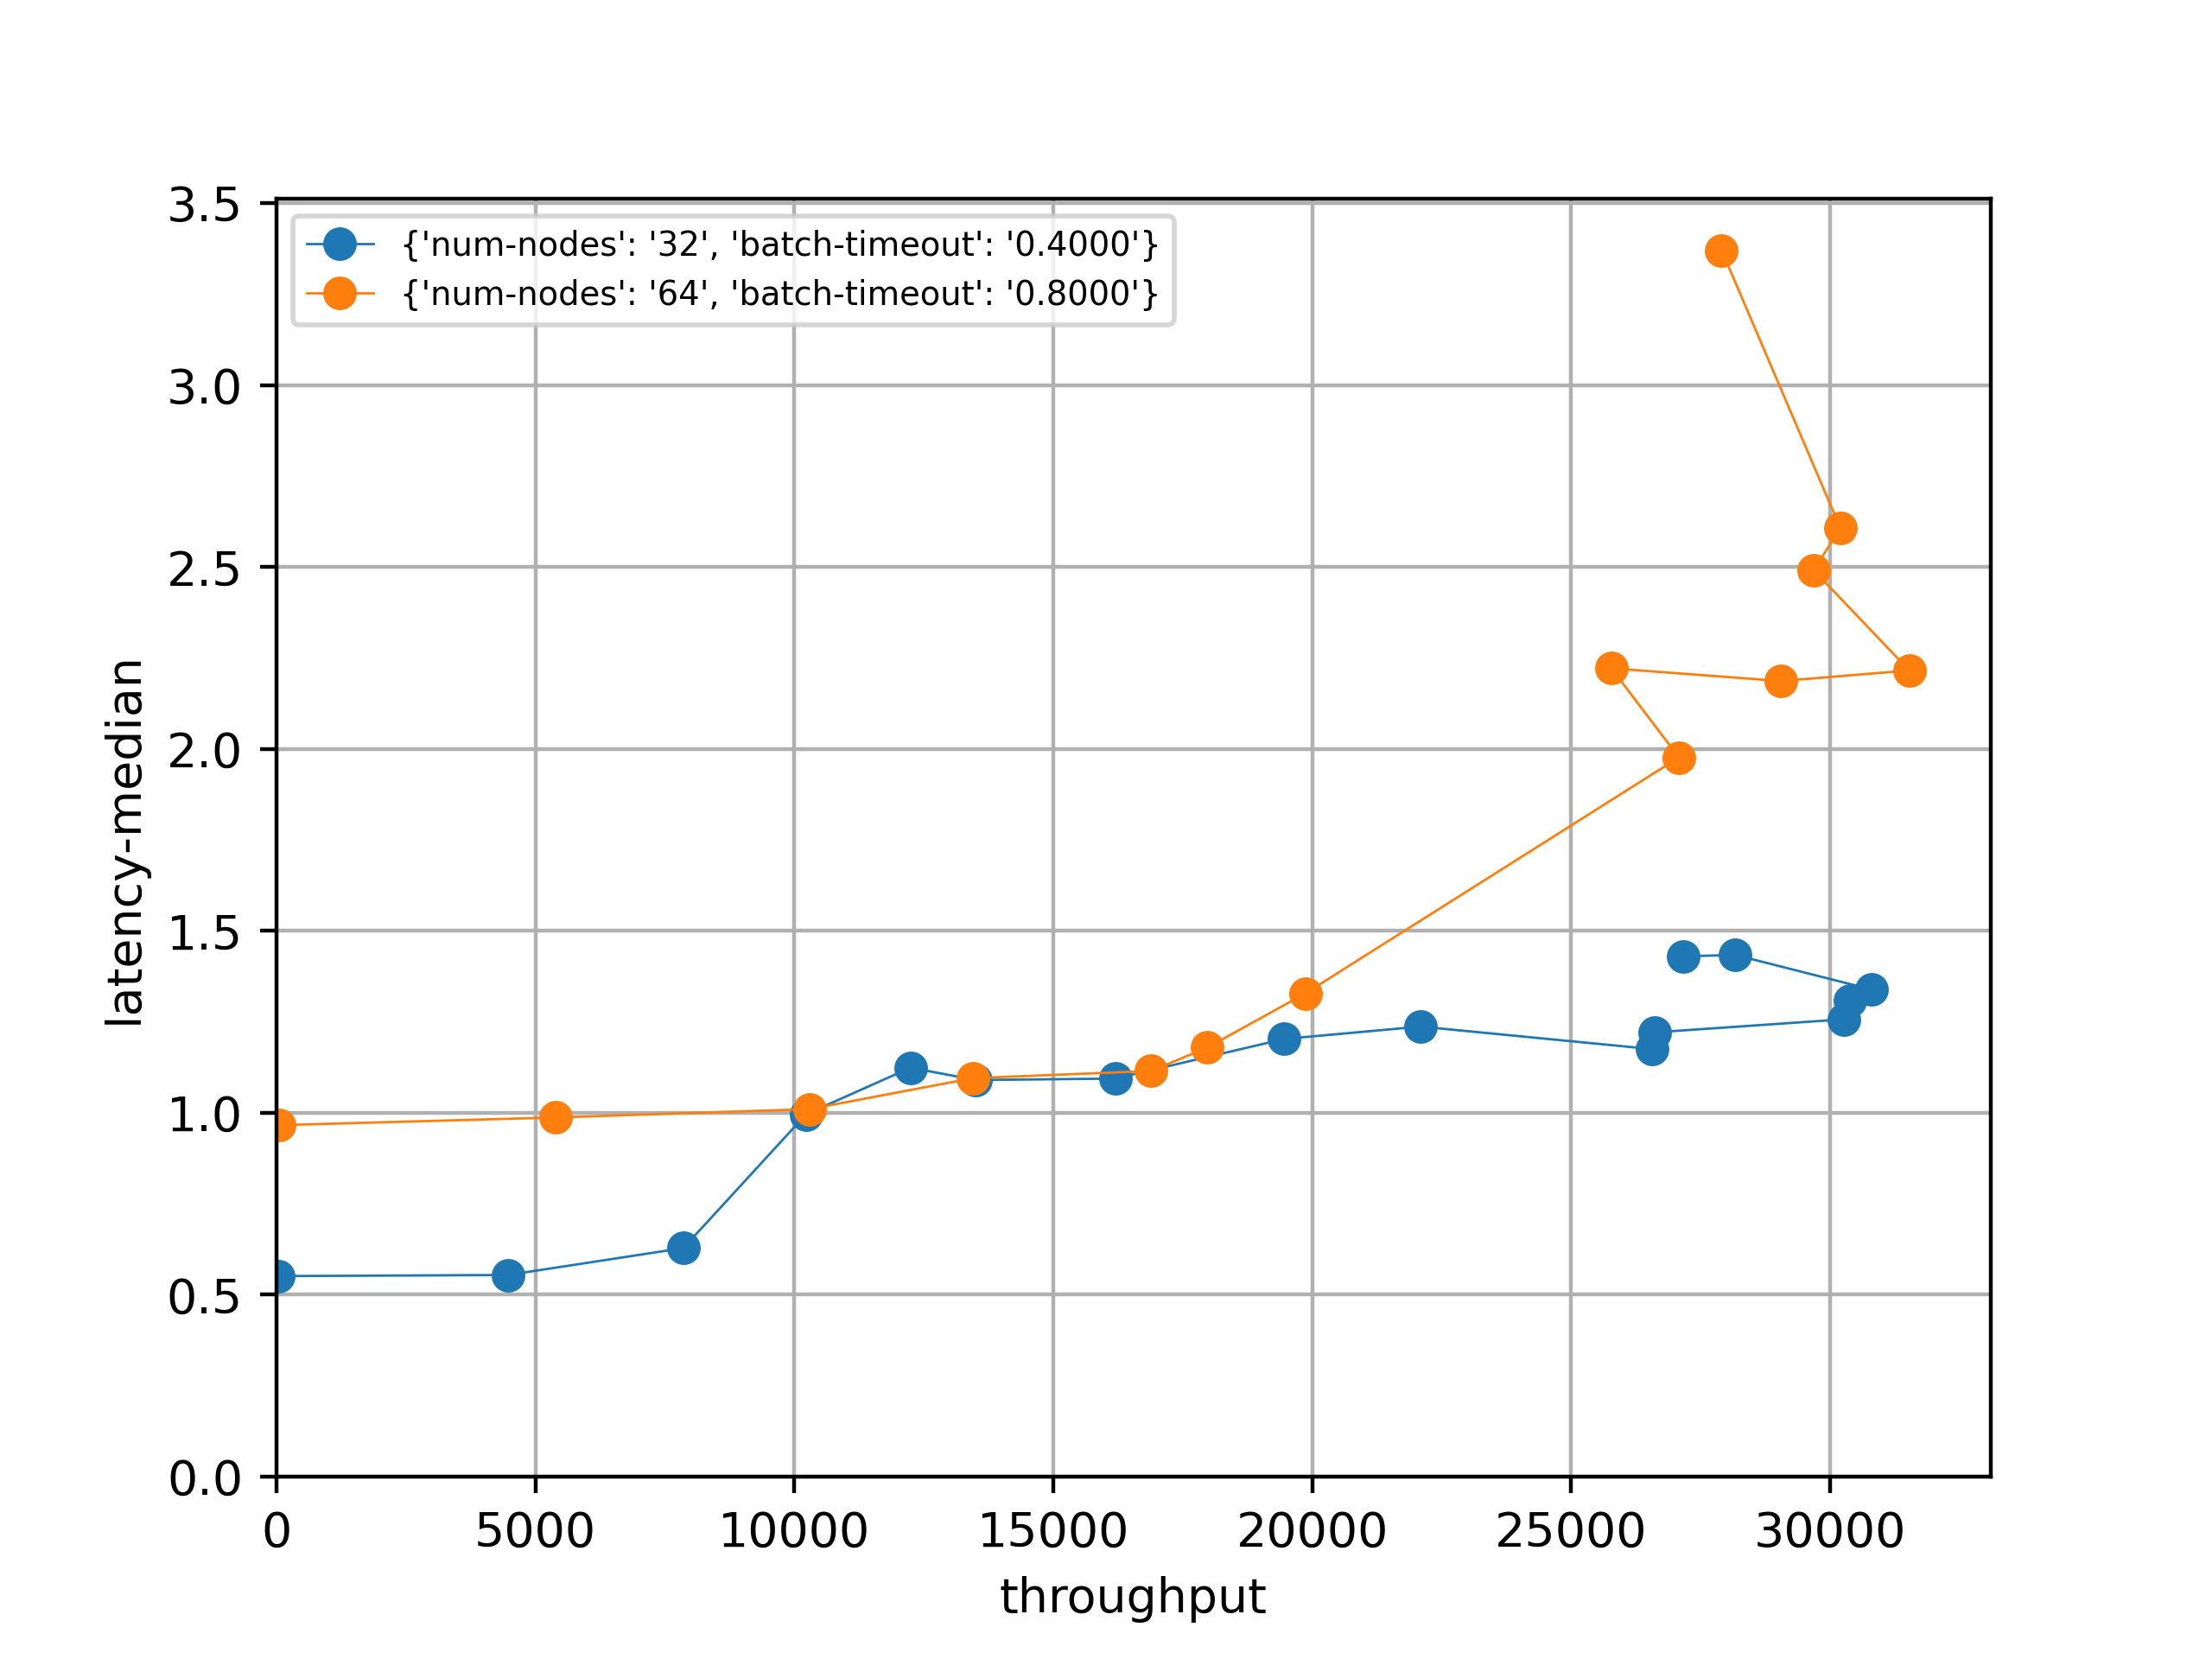
\includegraphics[width=0.79\textwidth]{figures/results-wan-final.png}
    \caption{\centering Median latency (in seconds) vs. throughput (in tx/s)\newline
    in a WAN deployment of 32 and 64 replicas.}
    \label{fig:eval-wan}
\end{figure}

\Cref{fig:eval-wan} shows Trantor's performance when deployed across the globe.
For 32 replicas, Trantor achieves a sub-second latency for throughputs of up to 10'000 tx/s,
and under a load of up to 8'000 concurrent clients (throughput of 4000' tx/s), Trantor's median ordering latency is as low as 0.5 seconds.
Trantor keeps a latency under 1.3 seconds until it reaches its peak throughput of above 30'000 tx/s with around 50'000 concurrent clients.
At this point, the system saturates and an increased number of clients only results in an increased latency.
When increasing the number of clients even further, even the throughput starts decreasing due to thrashing effects.
We chose the \param{BatchTimeout} of 0.4 seconds empirically,
as it provided the best results after a brief (and non-exhaustive) search of the parameter space.

A WAN deployment of 64 replicas yields slightly higher latency and, interestingly, a comparable peak throughput.
This suggests that the network bandwidth is not the bottleneck, at least for the 32-replica deployment.
Indeed, The average bandwidth used per replica at saturation is 16 MiB/s and 21 MiB/s respectively for the small and large scale deployment.

Another interesting phenomenon occurs at throughputs between 10'000 and ca. 17'000 tx/s, where both system sizes exhibit the same latencies.
We attribute this to the different setting of the \param{BatchTimeout} parameter for the two different system sizes,
as we increase the \param{BatchTimeout} at larger scale to 0.8 s to compensate for the higher message processing overhead.%
\footnote{Due to the rather large batch size limit of 2048 transactions,
most of the batches in our experiments are not completely full and are triggered by the \event{BatchTimeout}, especially before the system is saturated.}

\begin{figure}
    \centering
    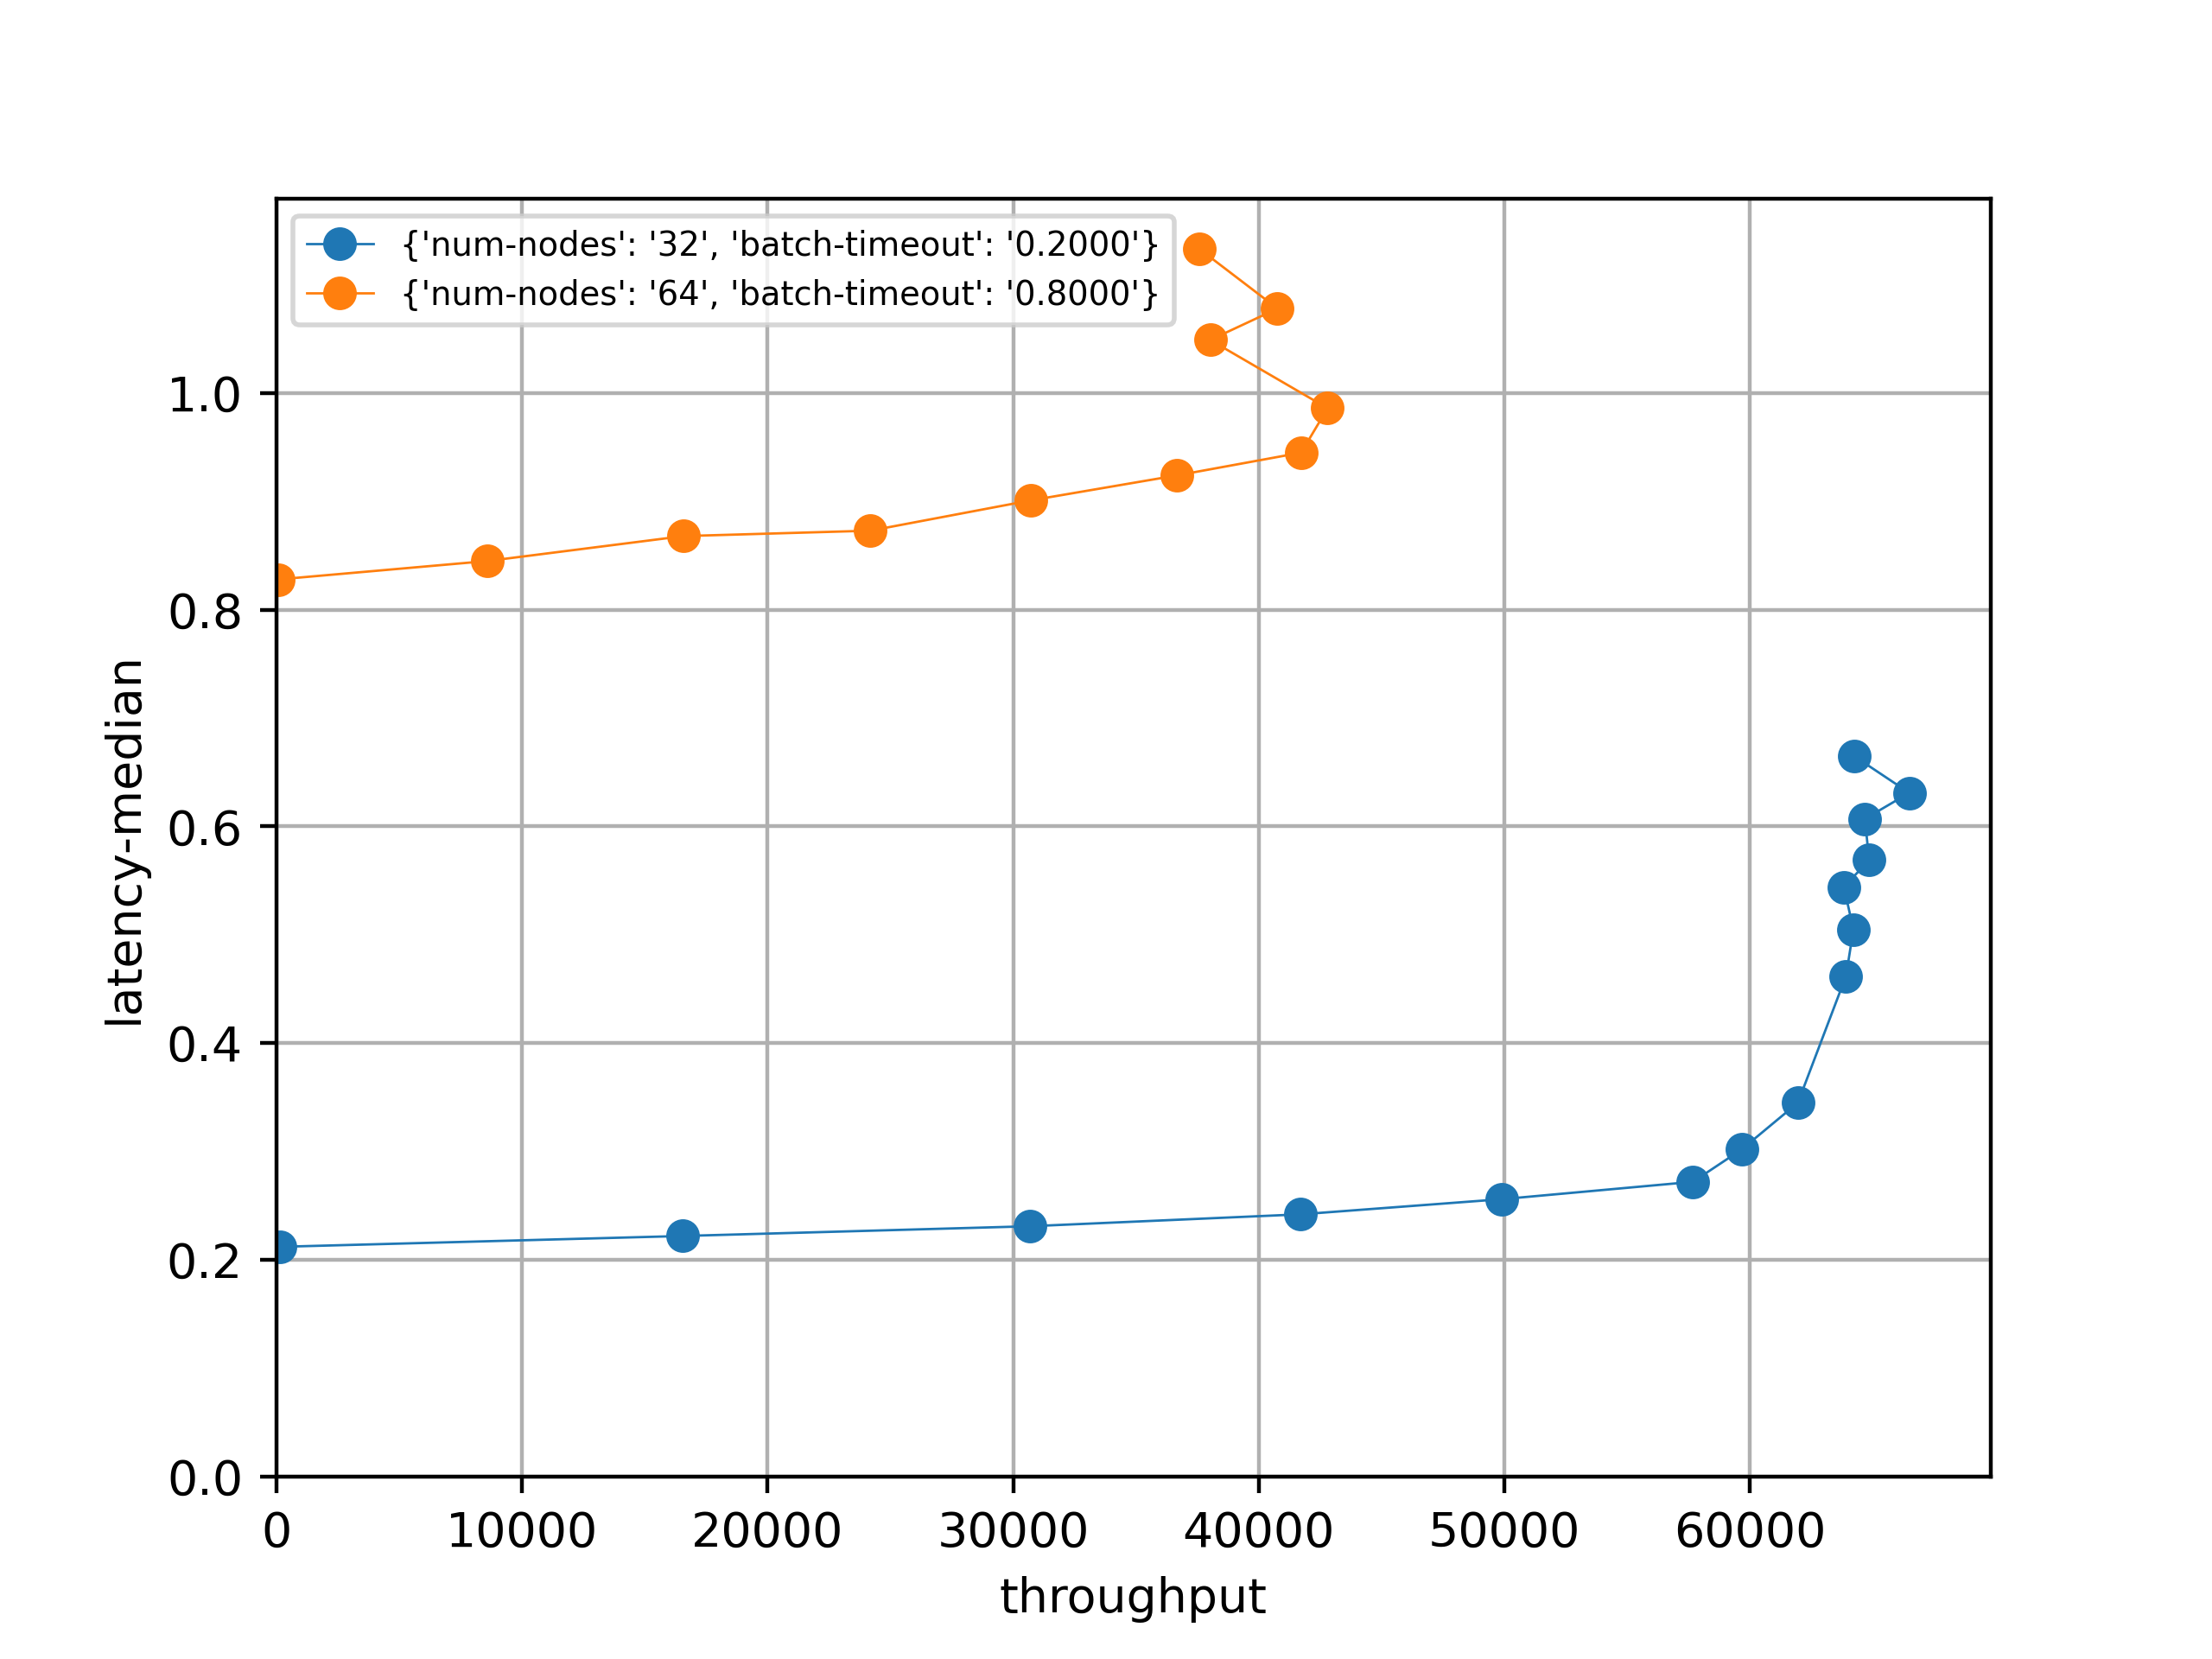
\includegraphics[width=0.79\textwidth]{figures/results-lan-final.png}
    \caption{\centering Median latency (in seconds) vs. throughput (in tx/s)
    in a LAN deployment of 32 and 64 replicas,
    for various segment lengths and \param{BatchTimeout} values.}
    \label{fig:eval-lan}
\end{figure}

% \paragraph{\param{SegmentLength} parameter.} Being heavily inspired by ISS \cite{iss},
% Trantor's ordering protocol subdivides each epoch into so-called segments.
% In a nutshell, a segment is a subset of sequence numbers within one epoch for which the same replica is disseminating and proposing a transaction batch
% (i.e., in our case, serves as the PBFT primary).
% The union of all segments makes up the whole epoch.
% The \param{SegmentLength} is the number of batches each replica needs to propose (and have the system agree upon) in each epoch.
% Thus, for example, for a \param{SegmentLength} of 2 and 32 replicas, the epoch length is 64
% and each replica proposes (concurrently with other replicas) 2 batches before the next epoch can start.

% Since Trantor creates a checkpoint at each epoch transition,
% shorter segments generally mean more checkpointing overhead and an increased good-case latency,
% as the system must wait more often for a checkpoint before starting a new epoch.
% However, longer epochs increase the risk of more replicas falling behind during one epoch
% and introducing instability in the system that might lead to thrashing, especially in large deployments.
% If a single replica is slow at, say, disseminating transaction batches,
% all other replicas need to wait for it at the end of the epoch,
% which has a significant impact on the latency of transactions waiting in the mempool.
% For all experiments except for one, we use a \param{SegmentLength} of 2.

\Cref{fig:eval-lan} shows Trantor's performance when deployed in a single datacenter with a fast network.
For 32 replicas, until the system starts becoming saturated at 60'000 tx/s, Trantor's latency is mostly under 0.25 seconds.
For a deployment of 64 replicas, throughput drops to 40'000 tx/s and latency increases to just below 1 second.
This is because each replica needs to wait for a larger quorum in order to make progress in both the dissemination and the ordering protocol.
Also, the overhead of ordering every transaction is higher, as each replica needs to send more outgoing messages and process more incoming ones.
This has a strong impact both on the network bandwidth (mostly for the dissemination component) and CPU load (mostly the ordering component).
We partially compensate for the higher CPU load by increasing the \param{BatchTimeout} to 0.8 seconds,
but it does not seem to be sufficient on a LAN.
We attribute this to a bandwidth bottleneck since, at saturation, both the small and large scale deployments
rarely exceed an average network transmission rate of 35 MiB/s per replica.

\subsection{Discussion}

In the following, we discuss some additional noteworthy aspects of Trantor's performance evaluation.

\paragraph{LAN Latency.}
When deployed in a single datacenter, Trantor's latency is higher than one might expect from a system deployed on such a fast network.
In fact, for 64 replicas, the LAN latency is almost as high as in the WAN.
This has two main reasons.

First, the algorithms used are not latency-optimal.
The very rudimentary implementation of the dissemination component adds an extra round-trip (quorum gathering) to the latency of PBFT.
This can, however, be alleviated by using better protocols for dissemination and ordering, e.g., as is done in Bullshark \cite{bullshark}.

Second, Trantor's current implementation focuses on feature-completeness, not on processing performance.
Therefore, it is very likely that local message processing also has a non-negligible contribution to overall transaction latency.

\paragraph{Transaction Deduplication.}
In a scenario like the above, a client might submit the same transaction to multiple replicas' mempools.
As described in \cref{sec:tx-deduplication}, the current implementation of Trnator would treat them as separate transactions,
lowering the effective throughput.
In our experiments, such duplication does not occur, since we also do not expect it to occur during normal operation in a real-world deployment.
Nevertheless, a slightly modified version of Trnator's dissemination and ordering components
can easily implement a deduplication mechanism \cite{mirbft,iss} to mitigate this issue.

\paragraph{Access Control.}
Trantor does not authenticate the sources of received transactions and implements no access control.
We believe this is not the task of the core of an SMR system and should be implemented on top of it.
Trantor provides all the necessary tools for the application to support access control, however.
The ordering component supports an optional external input validation mechanism (not discussed so far for simplicity),
allowing an early abortion of the ordering of transactions that an injected dependency considers invalid.
Our evaluation does not make use of it and thus also does not take into account it's potential overhead.

\paragraph{Unoptimized Implementation.}
Trantor's current implementation focuses on modularity and feature-completeness rather than on immediate performance optimization.
We prefer having smaller, well-encapsulated modules with simple yet meaningful interfaces
that significantly simplify reasoning about both their interaction and implementation.
For example, fetching missing transactions has a very simple interface (\event{RequestTransactions}/\event{ProvideTransactions}),
but its implementation is the most naive possible: requesting all transactions referenced by the certificate from all replicas that signed it,
introducing manyfold redundancy.

Our Go implementation also uses (for historical reasons) an extremely inefficient representation of messages based on Protocol Buffers,
where simple deserialization of a received message involves more than 10 (in some cases potentially more than 20) memory allocations.

Trantor achieves the presented performance despite these and many more inefficiencies.
More importantly, Trantor makes it easy to optimize each component separately in the future.
Even this document mentions several improvements that can be implemented in a future version of Trantor.
Trantor's architecture makes it easy to do so with only minimal modifications (if any at all) to the present system.
If deemed necessary, even optimizations that intrinsically require breaking abstraction boundaries
can be implemented in Trantor by replacing multiple involved components by a single, more integrated one.

\section{Conclusions}
\label{sec:conclusions}

Trantor is a state machine replication (SMR) system that allows an arbitrary application modeled as a deterministic state machine
to be deployed across multiple replicas in a fault-tolerant way.
Trantor’s design focuses on modularity.
We decompose the problem of SMR at the conceptual level into smaller sub-problems, each of which can be studied, reasoned about, and implemented separately.
We design the solution to each of these sub-problems as a separate component of Trantor.
In the future, it should be easy to replace or rearrange these components to adapt the system to varying requirements and new state of the art.

A preliminary good-case performance evaluation of Trnator shows very promising results
with a throughput in the tens of thousands tx/s and sub-second latency,
even when deployed over a WAN across the globe.
All this despite its simple implementation that still leaves a very large potential for performance optimization.

Trantor does not claim novelty in terms of protocols used or performance achieved.
In fact, the implementation of some of Trantor’s components is naive and sub-optimal compared to what is achievable in theory (and in practice).
It is not (yet) the point of Trantor to employ the most state-of-the-art component implementations, but to enable anyone to do so easily.
The ultimate goal is to be able to cherry-pick existing solutions to the multitude of sub-problems in SMR and flexibly combine them within one SMR system.

\newpage

\bibliographystyle{plain}
\bibliography{bibliography}

\end{document}
